\chapter{Desktop Teleoperated Surgical Training System}

In an effort to further advance the field of robotic-assisted surgery, researchers at MCI have developed a Desktop Teleoperated Surgical Training System. The system's design was heavily inspired by the da Vinci Research Kit (DVRK) and Raven II, with a focus on maximizing performance while minimizing cost. This system serves as the foundation for the research outlined in this paper, so an understanding of its design and architecture is essential.

\section{Overall System Architecture}

The system consists of two main components:

\begin{itemize}
    \item The Master Tool Manipulator (MTM)
    \item The Patient Side Manipulator (PSM)
\end{itemize}

\subsection{Master Tool Manipulator (MTM)}
The MTM is a serial-link manipulator that measures the operator's motion through a 7-DOF (degree-of-freedom) linkage, actuated by the user. It includes:

\begin{itemize}
    \item 3 DOFs for tracking overall system position (J0--J2)
    \item 4 DOFs for tracking gimbal position and state (G0--G3)
\end{itemize}

This allows the operator to communicate desired motions to the PSM. The J0--J2 DOFs dictate the endpoint position, while G0--G3 control endpoint orientation and state.

The MTM should allow for accurate interpretation of the operator's intended motion while also minimizing the force perceived by the operator. This perceived force requirement drove the design toward a gravity compensation system (GCS).

\subsection{Patient Side Manipulator (PSM)}
The PSM has 7 primary DOFs, divided into:

\begin{itemize}
    \item \textbf{Overall System Position:}
        \begin{itemize}
            \item Roll
            \item Pitch
            \item Insertion
        \end{itemize}
    \item \textbf{Surgical Instrument Control:}
        \begin{itemize}
            \item Instrument Roll
            \item Instrument Pitch
            \item Instrument Tilt
            \item Instrument Open/Close
        \end{itemize}
\end{itemize}

The system is actuated using:
\begin{itemize}
    \item Maxon brushless motors (for overall positioning)
    \item Servo motors (for instrument control)
\end{itemize}

Position feedback is provided by three 12-bit absolute optical encoders, and force reduction is achieved through:
\begin{itemize}
    \item Capstan drives (for roll and pitch axes)
    \item Rack-and-pinion (for insertion)
\end{itemize}

\begin{figure}[h]
    \centering
    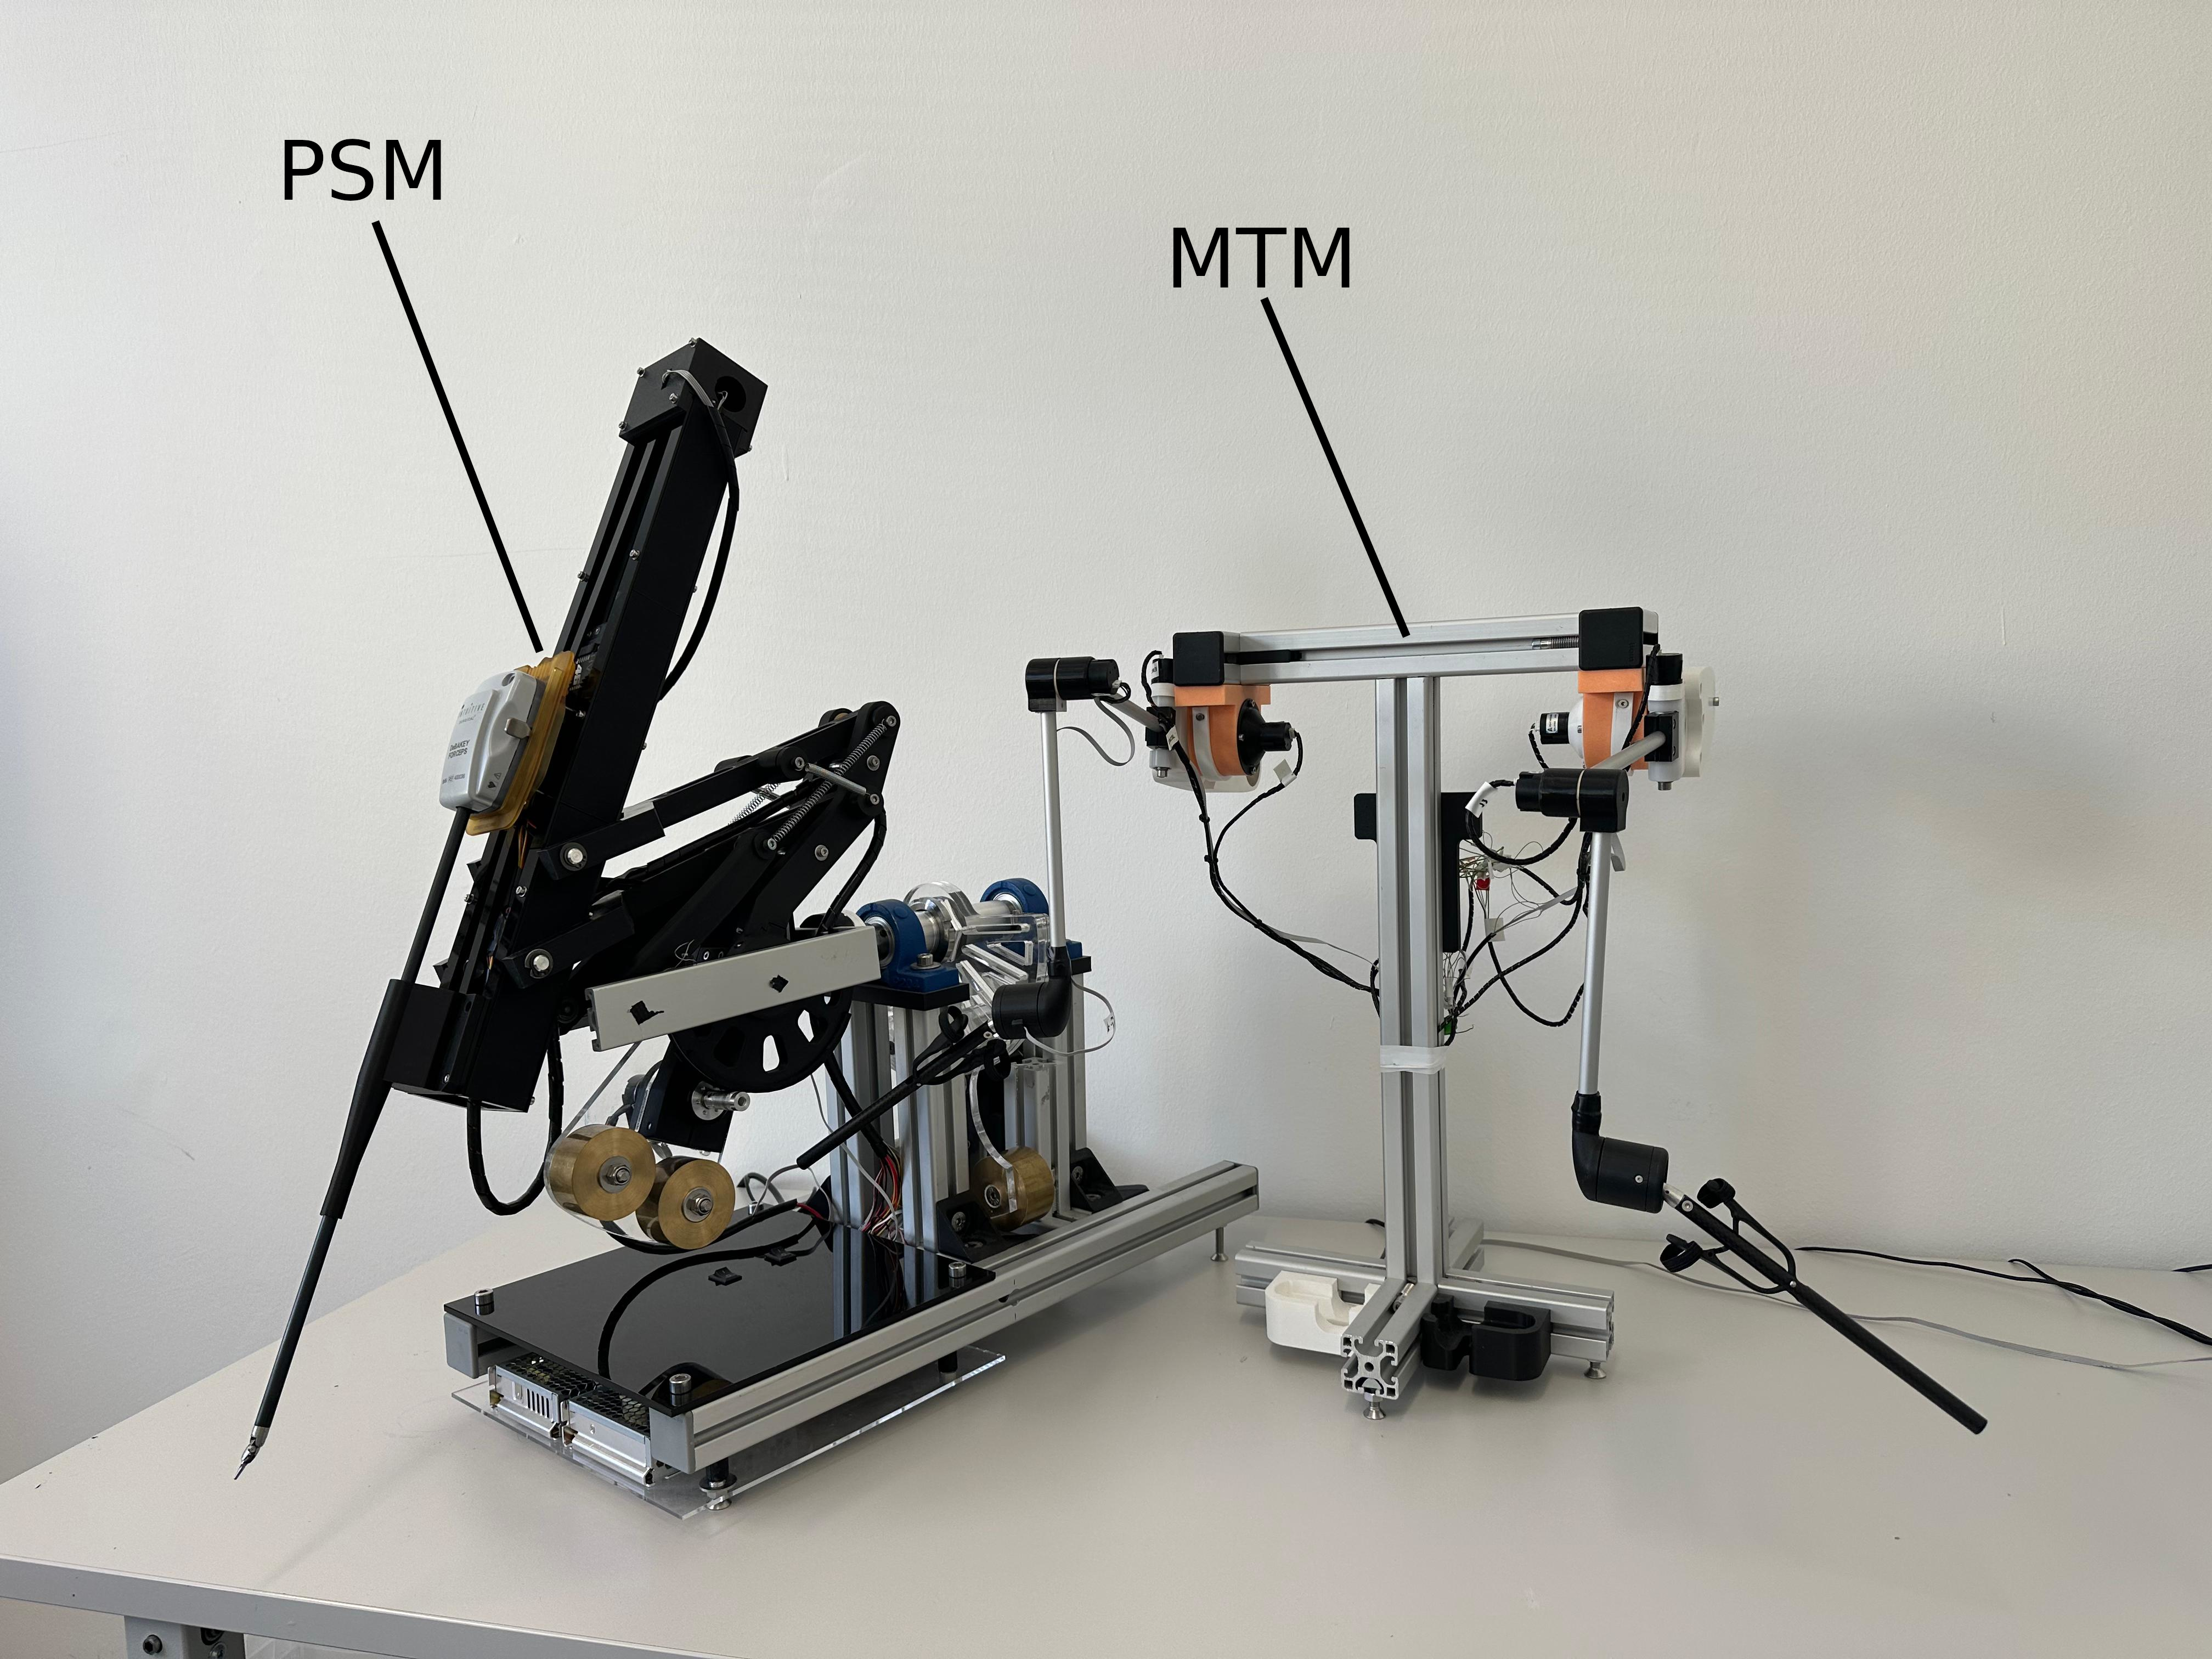
\includegraphics[width=0.75\linewidth]{figures/design/system_overview.png}
    \caption{Placeholder image of system}
    \label{fig:system_overview_placeholder}
\end{figure}


\section{MTM Mechanical Design}

The Master Tool Manipulator (MTM) can be separated into two subsystems:
\begin{itemize}
    \item Arm (J0-J2)
    \item Gimbal (G0-G3)
\end{itemize}

The arm subsystem refers to the overall architecture which is responsible for measuring the operator's position with respect to (w.r.t.) the global reference frame. Three revolute joints with internal optical encoders are coupled via rigid aluminum extrusions, allowing for accurate estimation of the overall system positioning in 3D space, as shown in Figure~\ref{fig:mtm_overview}.

\begin{figure}[h]
    \centering
    \includegraphics[width=0.75\linewidth]{figures/mtm_overview.png}
    \caption{Detailed depiction of the MTM's arm and wrist subsystems, with their individual components labeled.}
    \label{fig:mtm_overview}
\end{figure}

\subsection{Joints}
The arm of the manipulator consists of three revolute joints connecting the four links of the MTM arm. Table~\ref{tab:mtm_joints} summarizes these joints and provides a description of their function.

\begin{table}[h]
\centering
\caption{Summary and description of revolute (R) joints of the MTM's arm \cite{ref19,ref20}.}
\label{tab:mtm_joints}
\begin{tabular}{|c|c|l|p{8cm}|}
\hline
\textbf{MTM Joint} & \textbf{Joint Type} & \textbf{Joint Name} & \textbf{Description} \\
\hline
1 & R & Shoulder pitch & This joint moves the entire MTM and carries out pitch rotation similar to joint 3. \\
\hline
2 & R & Shoulder yaw & This joint is responsible for adduction and abduction movement of the operator. \\
\hline
3 & R & Elbow pitch & This joint is the second pitch joint of the MTM. Together with joint 1, it is responsible for up/down and forward/backward motion. \\
\hline
\end{tabular}
\end{table}

The design of these joints was driven by the requirement to minimize friction. Increased frictional forces in any of these joints would result in an increase in perceived force by the operator. As visible in Figure~\ref{fig:mtm_detailed}, roller bearings were utilized to minimize these frictional forces, and system mass was also reduced to lower both gravitational and inertial forces felt by the operator.

\begin{figure}[h]
    \centering
    \includegraphics[width=0.75\linewidth]{figures/mtm_detailed.png}
    \caption{Exploded view of the MTM components (excluding EWCU fixation) showing the updated training console design. Key improvements include: (1) circlip for axial safeguarding, (2) PTFE thrust washer to eliminate bearing clearance effects while maintaining low friction, and (3) reduced wear characteristics.}
    \label{fig:mtm_detailed}
\end{figure}


\section{MTM Electrical Architecture}

\subsection{System Overview}
The MTM (Master Tool Manipulator) electrical architecture was originally based around an Arduino Mega 2560 microcontroller that served as both the primary controller and system I/O interface. This configuration was later upgraded to a Teensy 4.1 microcontroller due to its superior performance and compatibility with ROS2 and micro-ROS frameworks.

The system incorporates multiple sensor subsystems to monitor and control the robotic arm's movements. Each side of the arm is equipped with sensors for:
\begin{itemize}
    \item Shoulder pitch (J0)
    \item Shoulder yaw (J1)
    \item Elbow pitch (J2)
    \item Wrist orientation (G0-G2)
    \item Grasper state (G3)
\end{itemize}

\subsection{Joint Subsystems (J0-J2)}
Joints J0-J2 are equipped with AEAT-6012-A06 12-bit absolute magnetic encoders (resolution: 4096 counts/revolution) directly coupled to each joint axis. These encoders provide a positional accuracy of $\pm 0.088^\circ$ ($360^\circ/4096$) per joint, enabling precise positional feedback for the control system.

\begin{itemize}
    \item \textbf{Shoulder Pitch (J0)}: Magnetic encoder provides precise feedback on shoulder pitch position
    \item \textbf{Shoulder Yaw (J1)}: Magnetic encoder measures shoulder yaw angle
    \item \textbf{Elbow Pitch (J2)}: Magnetic encoder monitors elbow pitch movement
\end{itemize}

The encoder signals are connected directly to the Teensy 4.1's digital I/O pins through a noise-resistant shielded cable assembly.

\subsection{Wrist Subsystem (G0-G3)}
The wrist subsystem underwent significant design evolution:
\begin{itemize}
    \item \textbf{Initial Design}: Utilized an MPU-6050 IMU (3-DOF) for wrist orientation sensing and a Hall effect sensor for grasper state detection
    \item \textbf{Issues Encountered}: Noticeable drift occurred in the IMU during prolonged operation
    \item \textbf{Final Implementation}: Replaced with analog potentiometers for wrist position detection (G0-G2) while retaining the Hall effect sensor for grasper state detection (G3)
\end{itemize}

The MPU-6050 IMU provided the following measurement capabilities:
\begin{itemize}
    \item 3-axis accelerometer ($\pm 2/4/8/16$ g configurable)
    \item 3-axis gyroscope ($\pm 250/500/1000/2000^\circ$/s configurable)
\end{itemize}

\subsection{Connectivity}
All wrist sensors (G0-G3) connect to the Teensy 4.1's analog I/O pins through a 7-strand flat flexible cable (FFC) with the following specifications:
\begin{itemize}
    \item Pitch: 0.5mm
    \item Current rating: 0.3A per conductor
    \item Voltage rating: 50V
    \item Temperature range: $-40^\circ$C to $+105^\circ$C
\end{itemize}

\subsection{Grip Subsystem}
The grip detection system utilizes a Hall effect sensor to measure the position between the index finger and thumb components. Key characteristics include:
\begin{itemize}
    \item Sensing range: $\pm 50$mm
    \item Resolution: 0.1mm
    \item Output: Analog voltage (0-3.3V)
\end{itemize}

\section{PSM Mechanical Design}

\subsection{Overview}
The Patient-Side Manipulator (PSM) mechanical architecture is a 7-degree-of-freedom (DOF) robotic system designed to replicate surgical instrument movements with high precision. The design is fundamentally inspired by the da Vinci Surgical System's remote center of motion (RCM) mechanism, which maintains a fixed pivot point at the surgical incision site - a critical feature for minimally invasive surgery. The PSM can be divided into five primary subsystems:

\begin{itemize}
    \item Superstructure and base
    \item Roll (yaw) axis
    \item Pitch axis
    \item Insertion axis
    \item Tool cart and end effector
\end{itemize}

\subsection{Superstructure}
The superstructure serves as the foundational framework, constructed from 80/20 aluminum extrusion for both rigidity and modularity. This design provides:
\begin{itemize}
    \item Structural stability for the entire system
    \item Mounting points for all electromechanical components
    \item Vibration damping through its triangulated geometry
    \item Accessibility for maintenance and upgrades
\end{itemize}

The aluminum extrusion profile (40mm × 40mm, series 8) was selected for its excellent strength-to-weight ratio and compatibility with standard motion components.

\subsection{Roll (Yaw) Axis}
The roll axis implements a revolute joint providing $\pm$90$^\circ$ of rotation about the vertical axis, corresponding to the da Vinci system's first DOF.

\begin{itemize}
    \item \textbf{Drive System}: Maxon EC-4pole 30 brushless DC motor (50W) coupled to a 20:1 Capstan drive
    \item \textbf{Transmission}: Zero-backlash Capstan drive (0.1 arc-minute repeatability)
    \item \textbf{Bearing System}: Two NSK LH-series linear bearing blocks supporting a 16mm ground aluminum shaft
    \item \textbf{Position Sensing}: Broadcom HEDS-5540 optical encoder (500 CPR)
    \item \textbf{Safety}: Omron D2F-L-A1 limit switches at $\pm$90$^\circ$ travel limits
\end{itemize}

The roll axis terminates in an aluminum fork structure that supports both the pitch and insertion axes, maintaining the kinematic chain.

\subsection{Pitch Axis}
The pitch axis replicates the da Vinci's characteristic parallelogram mechanism, which creates a virtual RCM approximately 50mm distal to the joint - matching typical trocar insertion depths.

\begin{itemize}
    \item \textbf{Mechanism}: Dual-parallelogram linkage with 3D-printed ABS components
    \item \textbf{Drive System}: Maxon EC-4pole 30 motor with identical 20:1 Capstan drive
    \item \textbf{Range of Motion}: $\pm$45$^\circ$ from neutral position
    \item \textbf{Advantages}:
        \begin{itemize}
            \item Maintains constant instrument orientation during arm motion
            \item Creates natural RCM without complex constrained mechanisms
            \item Reduces shear forces at the incision point
        \end{itemize}
\end{itemize}

The 3D-printed design (Prusa MK3S+, 0.15mm layer height) was chosen for rapid prototyping and weight reduction, with critical joints reinforced with stainless steel pins.

\subsection{Insertion Axis}
The prismatic insertion axis provides 200mm of linear travel, corresponding to the da Vinci's third DOF.

\begin{itemize}
    \item \textbf{Drive Mechanism}: HV7346MG servo (modified for continuous rotation) with rack-and-pinion transmission
    \item \textbf{Guide System}: IGUS drylin linear rails (model RJ4JP-01-08)
    \item \textbf{Position Sensing}: Integrated optical encoder with 0.1mm resolution
    \item \textbf{Safety}: Dual Omron limit switches at travel extremes
\end{itemize}

The rack-and-pinion system (module 0.5, 20$^\circ$ pressure angle) provides 96.5\% efficiency while maintaining the compact form factor required for surgical applications.

\subsection{Tool Cart and End Effector}
The tool cart integrates four degrees of freedom in a package matching Intuitive Surgical's instrument specifications:

\begin{itemize}
    \item \textbf{Actuation}: Four MG966R servos with spring-loaded coupling mechanisms
    \item \textbf{Functions}:
        \begin{itemize}
            \item Instrument roll ($\pm$90$^\circ$)
            \item Wrist pitch ($\pm$85$^\circ$)
            \item Wrist yaw ($\pm$85$^\circ$)
            \item Grasper actuation (0-100\%)
        \end{itemize}
    \item \textbf{Instrument Interface}: Compatible with Intuitive Surgical EndoWrist\textsuperscript{\textregistered} tools
    \item \textbf{Coupling Mechanism}: Fail-safe magnetic coupling with 5N retention force
\end{itemize}

\subsection{Remote Center of Motion Implementation}
The PSM's mechanical architecture replicates the da Vinci system's key innovation - the passive RCM mechanism. This is achieved through:

\begin{itemize}
    \item \textbf{Parallelogram Linkage}: Mathematically constrains motion to a fixed point
    \item \textbf{Kinematic Design}: Aligns axes to intersect at the RCM point
    \item \textbf{Clinical Benefits}:
        \begin{itemize}
            \item Minimizes tissue trauma at incision site
            \item Provides intuitive instrument control
            \item Reduces fulcrum effect during manipulation
        \end{itemize}
\end{itemize}


\section{PSM Electrical Architecture}

\subsection{System Overview}
The Patient-Side Manipulator (PSM) electrical architecture is designed to meet stringent surgical robotic requirements, including:
\begin{itemize}
    \item Sub-millimeter positional accuracy ($\pm$0.2mm at instrument tip)
    \item High dynamic response (bandwidth > 10Hz for all axes)
    \item Fail-safe operation with redundant position verification
    \item Low-latency control loops ($<$1ms cycle time)
\end{itemize}

The system implements a distributed control architecture centered around a Teensy 4.1 microcontroller (600MHz ARM Cortex-M7), chosen for its:
\begin{itemize}
    \item Real-time performance capabilities
    \item Extensive I/O options (28 PWM channels, 16 analog inputs)
    \item Native USB 2.0 support for ROS2 integration
    \item FPU support for advanced control algorithms
\end{itemize}

\subsection{Position Sensing System}
\subsubsection{Primary Joint Sensing}
\begin{itemize}
    \item \textbf{Roll/Yaw Axis}: Broadcom HEDS-5540 optical encoder (500 CPR) with quadrature decoding
    \item \textbf{Pitch Axis}: Broadcom HEDS-5540 optical encoder (500 CPR)
    \item \textbf{Insertion Axis}: AMS AS5047P magnetic encoder (14-bit resolution, 0.022$^\circ$ accuracy)
\end{itemize}

\subsubsection{Secondary Verification}
\begin{itemize}
    \item Omron D2F-L-A1 mechanical limit switches at all travel extremes
    \item Current sensing via INA219 shunt monitors (0.5\% accuracy)
    \item Thermal monitoring on all motor drivers
\end{itemize}

\subsection{Motor Drive System}
\subsubsection{Main Axes Actuation}
\begin{table}[h]
\centering
\caption{Main Axes Drive Specifications}
\begin{tabular}{|l|c|c|c|}
\hline
\textbf{Parameter} & \textbf{Roll} & \textbf{Pitch} & \textbf{Insertion} \\ \hline
Motor & Maxon EC-4pole 30 & Maxon EC-4pole 30 & HV7346MG \\
Voltage & 24V & 24V & 12V \\
Continuous Current & 2.5A & 2.5A & 3.2A \\
Peak Torque & 50mNm & 50mNm & 15kg-cm \\
Driver & MD13S Cytron & MD13S Cytron & MD13S Cytron \\
Control Mode & PID Velocity & PID Position & PID Position \\
Bandwidth & 500Hz & 500Hz & 300Hz \\ \hline
\end{tabular}
\end{table}

\subsubsection{Servo Control Implementation}
The wrist subsystem utilizes four MG966R servos modified for continuous rotation and external position control:
\begin{itemize}
    \item \textbf{Control Method}: PWM (1-2ms pulse width) with 12-bit resolution
    \item \textbf{Position Feedback}: Internal potentiometer (10k$\Omega$, 300$^\circ$ range)
    \item \textbf{External Verification}: AS5600 magnetic encoders on output shafts
    \item \textbf{Spring Coupling}: 0.5N/mm preloaded springs ensure zero backlash
\end{itemize}

\subsection{Safety and Calibration}
The system implements a comprehensive safety architecture:
\begin{itemize}
    \item Dual-channel limit switch verification (mechanical + optical)
    \item Watchdog timer (100ms timeout) on all motor drivers
    \item Current limiting at both driver and software levels
    \item Automatic homing sequence on startup:
    \begin{enumerate}
        \item Seek limit switch at reduced velocity (10\% max)
        \param{Back off 5mm from limit}
        \item Establish encoder zero position
    \end{enumerate}
\end{itemize}

\subsection{Control Architecture}
The Teensy 4.1 implements the following control scheme:
\begin{itemize}
    \item \textbf{Sampling Rate}: 1kHz for all critical loops
    \item \textbf{Algorithm}: Adaptive PID with velocity feedforward
    \item \textbf{Communication}:
    \begin{itemize}
        \item ROS2 interface (micro-ROS) @ 100Hz
        \item CAN bus for motor drivers (1Mbps)
        \item I$^2$C for sensors (400kHz fast mode)
    \end{itemize}
    \item \textbf{State Estimation}: Kalman filter combining encoder and IMU data
\end{itemize}

\subsection{Power Distribution}
\begin{itemize}
    \item \textbf{Main Bus}: 24V DC (Mean Well LRS-350-24)
    \item \textbf{Logic Power}: 5V/3A buck converter (TI TPS5430)
    \item \textbf{Protection}:
    \begin{itemize}
        \item Polyfuses on all outputs
        \item TVS diodes for surge protection
        \item Star grounding for noise reduction
    \end{itemize}
\end{itemize}

\section{System Software Architecture}
\label{sec:software_architecture}

As noted earlier in this paper, the initial software framework was implemented in an Arduino C-based environment. While the system has since been migrated to a ROS 2 architecture, the original implementation remains relevant for context and reference.

The software was divided into two primary components: the \textbf{Master Tool Manipulator (MTM)} software and the \textbf{Patient Side Manipulator (PSM)} software. These subsystems worked in tandem to enable real-time teleoperation, with the MTM capturing user inputs and the PSM replicating movements precisely.

\subsection{MTM Software}
The MTM software was responsible for:

\begin{enumerate}
    \item \textbf{Sensor Data Acquisition}:
    \begin{itemize}
        \item Reading six absolute magnetic encoders, two IMUs (Inertial Measurement Units), and two Hall effect sensors (eight sensor values per MTM arm)
        \item Distinguishing between left and right-arm data for independent kinematic processing
    \end{itemize}
    
    \item \textbf{Forward Kinematics}:
    \begin{itemize}
        \item Calculating the system's position and orientation from raw sensor data
        \item Smoothing noisy signals using low-pass filters (\texttt{LPFilter.ino}, \texttt{LPFilter\_Encoder.ino})
    \end{itemize}
    
    \item \textbf{Data Processing and Safety}:
    \begin{itemize}
        \item Detecting abrupt movements via spike detection logic (\texttt{spikeDetection.ino})
        \item Monitoring sensor overflow conditions (\texttt{OverFlowDetection.ino})
    \end{itemize}
    
    \item \textbf{Communication}:
    \begin{itemize}
        \item Relaying processed kinematic data to the PSM via serial communication
        \item Packaging data with start/end markers for robust parsing (\texttt{recvWithStartEndMarkers.ino})
    \end{itemize}
\end{enumerate}

\textbf{Key files included}:
\begin{itemize}
    \item \texttt{MT\_MTM.ino}: Central coordination, subsystem integration, and communication with the Arduino Mega
    \item \texttt{KinematicCalc\_L/R.ino}: Arm-specific forward kinematics for joint angle derivation
    \item \texttt{readIMU.ino} \& \texttt{readEncoder.ino}: IMU quaternion and encoder position data handling
\end{itemize}

\subsection{PSM Software}
The PSM software replicated MTM movements using:

\begin{enumerate}
    \item \textbf{Data Reception and Parsing}:
    \begin{itemize}
        \item Extracting target positions from serial messages (\texttt{parseData.ino})
    \end{itemize}
    
    \item \textbf{Closed-Loop Control}:
    \begin{itemize}
        \item Executing PID control for motor actuation (\texttt{PIDupdate.ino})
        \item Implementing ramp-up routines for smooth motion initiation (\texttt{RampUp\_Homing.ino})
    \end{itemize}
    
    \item \textbf{Safety and Calibration}:
    \begin{itemize}
        \item Collision detection via limit switches (\texttt{CheckCol.ino})
        \item Reference drives for incremental encoders (joints 1--3) to establish absolute positioning post-startup
        \item Tool manipulation routines (\texttt{Catch\_Tool.ino}) and PWM frequency tuning (\texttt{setPwmFrequency.ino})
    \end{itemize}
\end{enumerate}

\section{System Kinematics and Coordinate Frames}

\section{System PID Controller Design}


